
\chapter{INTRODUCCIÓN}

\section{Objetivo}
El objetivo de esta práctica es la resolución de un laberinto de 5x5 casillas, en el que la posición de las paredes, se desconoce a priori y en el que las casillas tienen un tamaño de 20x20 cm. Además de resolver el laberinto, es decir, llegar a una casilla de salida cuya posición se desconoce. Una vez que se haya encontrado la casilla de salida, volver a la casilla de entrada por el camino más corto posible.

\begin{itemize}
  \item Movimientos: Desplazamiento hacia delante, hacia atrás, giro a la izquierda y giro a la derecha
  \item Detección: Detección de paredes mediante el uso de sensores Sharp y ultrasonidos, y detección de color mediante el uso de sensores CNY70.
  \item Recogida de información: Se recoge información desde los sensores Sharp, CNY70 y el ultrasonidos.
  \item Algoritmo de resolución del laberinto: Se tiene una jerarquía de movimientos, estando en primer lugar, moverse a la derecha, luego al frente y por último a la izquierda. Todos estos movimientos se van guardando en una pila para que según se vaya avanzando en el laberinto en la pila sólo queden los movimientos que permiten alcanzar la casilla final, para que haciendo los movimientos inversos a los que están en la pila, el robot pueda volver a llegar a la casilla inicial por el camino más corto.
  \item Monitorización de información: La monitorización de la información se realiza a través de la aplicación móvil, que muestra la posición del robot en el laberinto junto con el nivel de batería restante, entre otras cosas.

\end{itemize}


\section{Hardware empleado}
En el diseño final se han utilizado los siguientes componentes:

\begin{itemize}
  \item CNY70: Sensor que mide la intensidad de la luz, permitiendo distinguir colores.
  \item Ultrasonidos: Sensor que permite calcular distancias mediante la producción de sonidos y su rebote.
  \item Sharp: Sensor que permite calcular las distancias mediante el uso de un haz de luz.
  \item HC-06 (Bluetooth): Módulo que permite leer y escribir datos mediante el puerto serie.
  \item Motores DC: Elemento mecánico que permite el movimiento.
  \item LED: Elemento electrónico que se ilumina con el paso de la corriente.
  \item Batería: Proporciona una fuente de alimentación externa.
\end{itemize}

\subsection{Arduino Leonardo}

Para ello, se utilizará una placa Arduino Leonardo, un ordenador personal y un móvil. A través del ordenador, se le descargará en la placa el programa para resolver el laberinto, una vez realizada la descarga del programa, se enlaza mediante Bluetooth la placa y un dispositivo móvil, donde se podrá ver la posición del robot en el laberinto y otros datos interesantes como el porcentaje de batería restante.

\subsection{Sensores}
\begin{itemize}
  \item CNY70: Su uso es necesario para comprobar el paso de una casilla a otra así como para comprobar si se ha llegado a la casilla de salida o no.
  \item Sharp: Se usa para detectar la existencia de paredes laterales.
  \item Ultrasonidos: Se usa para detectar la existencia de paredes frontales.
\end{itemize}

\subsection{Actuadores}
\begin{itemize}
  \item Interruptor: El interruptor es necesario para encender la placa.
\end{itemize}

\subsection{Elementos de comunicación}
\begin{itemize}
  \item HC-06: El conector Bluetooth se usa para mandar información a la app móvil para que en ésta se vean el nivel batería y la posición en el laberinto.
\end{itemize}

\subsection{Alimentación}
\begin{itemize}
  \item Batería de 6 pilas AA: Sirve para alimentar la placa.
\end{itemize}

\subsection{Justificación}
Se consideran que estos elementos son los mínimos imprescindibles para una correcta resolución del laberinto, ya que, desde un primer momento, el hecho de buscar un diseño similar al de un coche, teníamos claro que el ultrasonidos iría colocado en el lugar de los faros delanteros y por lo tanto, el uso de los servos resulta totalmente prescindible. Por otra parte, tampoco se usa el conector Bluetooth para el PC por estar utilizando una aplicación móvil.

\subsection{Resumen de Pines}
\begin{table}[h!]
  \centering
  \begin{tabular}{cc}

      \begin{tabular}{|c|c|}
        \hline
        PIN & ELEMENTO \\ \hline
        A5 & CNY Trasero \\ \hline
        A0 & CNY Izquierdo \\ \hline
        A1 & CNY Derecho \\ \hline
        A8 & Sharp Izquierdo \\ \hline
        A4 & Sharp Derecho \\ \hline
        RX, TX & Bluetooth \\ \hline
        A3 & Ultrasonidos \\ \hline
        12 & LED1 \\ \hline
        13 & LED2 \\ \hline
        11 & LED3 \\ \hline
        A6 & \% Batería \\ \hline

      \end{tabular}
    &  \vcenteredhbox{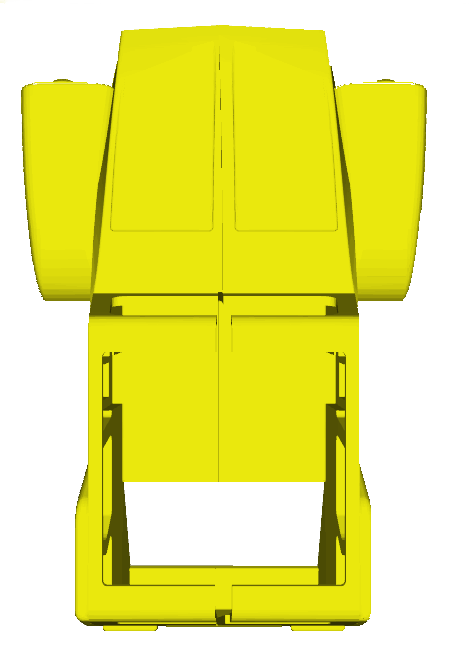
\includegraphics[scale=0.25]{img/CapraCenital.png}}\\
  \end{tabular}
  \caption{Resumen de los elementos y sus respectivos pines}
  \label{}
\end{table}



\section{Software empleado}
\subsection{Arduino IDE}
Resulta imprescindible el uso de este software por motivos obvios, gracias a él se le mandan los programas a la placa de Arduino. En nuestro caso, era también necesario para importar la librería externa que contiene la implementación de las estructuras de datos de la STL de C++ en Arduino, aunque ésto se detallará más adelante.

\subsection{React-Native}
\textit{React-Native} es una librería de Javascript que permite la creación de aplicaciones que tengan una apariencia nativa en el correspondiente sistema operativo móvil, en este caso en Android y iOS, usando un mismo código. ¿Por qué usar un móvil y no un PC? La respuesta viene dada con dos componentes, el primero la portabilidad y el segundo, la potencia.

Comenzando por la portabilidad, es evidente que es muchísimo más fácil transportar un móvil que un ordenador portátil, de esta forma, ante la posibilidad de tener que hacer presentaciones, sólo haría falta el robot y el móvil, ya que la placa de Arduino poseer una memoria flash, llevaría cargado el programa previamente. En cuanto a la potencia, la realidad es que en los últimos años la tecnología móvil ha avanzado lo suficiente como para igualar en ciertos aspectos al ordenador portátil, por tanto, si tuviesemos que mandar a realizar unos cálculos ya sea al ordenador o al móvil, como por ejemplo, calcular el camino de vuelta más corto usando el algoritmo de Dijkstra no habría tanta diferencia entre que lo haga un móvil o un ordenador.

Y, por otro lado, está el factor didáctico. \textit{React-Native} es una librería con un gran empuje en los últimos años y, de cara a aumentar nuestra formación en otras tecnologías, resultaba bastante interesante aprender lo más actual en el mundo empresarial.

\subsection{\LaTeX}
El hecho de utilizar \LaTeX \ era obligatorio en nuestra opinión para dotar a esta memoria de un aspecto académico, gracias en gran medida al paquete TikZ que permite la creación de gráficos vectoriales en \LaTeX \ con una gran versatilidad. Este paquete permite, por ejemplo, la creación de diagramas de Gantt, de diagramas de casos de uso o de diagramas de flujo.
